\documentclass[11pt,aspectratio=169]{beamer}
\usetheme{Madrid}

% ======================= PACKAGES =======================
\usepackage{graphicx}
\usepackage{booktabs}
\usepackage{adjustbox}
\usepackage{multicol}
\usepackage{amsmath}
\usepackage{amssymb}
\usepackage{tikz}
\usetikzlibrary{arrows,shapes,positioning,shadows,trees}
\usepackage{listings}
\usepackage{xcolor}

% ======================= COLOR DEFINITIONS =======================
% Primary color scheme: Blue/Teal for Digital Finance
\definecolor{dfblue}{RGB}{0,102,204}
\definecolor{dfteal}{RGB}{0,153,153}
\definecolor{dfcyan}{RGB}{51,187,204}
\definecolor{dflightblue}{RGB}{153,204,255}
\definecolor{dflightblue2}{RGB}{173,214,255}
\definecolor{dflightblue3}{RGB}{193,224,255}
\definecolor{dflightblue4}{RGB}{213,234,255}

% Accent colors for finance applications
\definecolor{dfgreen}{RGB}{44, 160, 44}
\definecolor{dfred}{RGB}{214, 39, 40}
\definecolor{dforange}{RGB}{255, 127, 14}
\definecolor{dfgray}{RGB}{127, 127, 127}

% Utility colors
\definecolor{lightgray}{RGB}{240, 240, 240}
\definecolor{midgray}{RGB}{180, 180, 180}
\definecolor{codebg}{RGB}{245, 245, 245}

% ======================= THEME CUSTOMIZATION =======================
% Apply Digital Finance color scheme to Madrid theme
\setbeamercolor{palette primary}{bg=dflightblue3,fg=dfblue}
\setbeamercolor{palette secondary}{bg=dflightblue2,fg=dfblue}
\setbeamercolor{palette tertiary}{bg=dfteal,fg=white}
\setbeamercolor{palette quaternary}{bg=dfblue,fg=white}

\setbeamercolor{structure}{fg=dfblue}
\setbeamercolor{section in toc}{fg=dfblue}
\setbeamercolor{subsection in toc}{fg=dfteal}
\setbeamercolor{title}{fg=dfblue}
\setbeamercolor{frametitle}{fg=dfblue,bg=dflightblue3}
\setbeamercolor{block title}{bg=dflightblue2,fg=dfblue}
\setbeamercolor{block body}{bg=dflightblue4,fg=black}

% Remove navigation symbols for cleaner look
\setbeamertemplate{navigation symbols}{}

% Clean itemize/enumerate
\setbeamertemplate{itemize items}[circle]
\setbeamertemplate{enumerate items}[default]

% Margins for readability
\setbeamersize{text margin left=8mm,text margin right=8mm}

% ======================= LISTINGS CONFIGURATION =======================
% Python code style
\lstdefinestyle{pythonstyle}{
    language=Python,
    basicstyle=\ttfamily\footnotesize,
    keywordstyle=\color{dfblue}\bfseries,
    stringstyle=\color{dforange},
    commentstyle=\color{dfgray}\itshape,
    numberstyle=\tiny\color{dfgray},
    numbers=left,
    numbersep=5pt,
    backgroundcolor=\color{codebg},
    showspaces=false,
    showstringspaces=false,
    showtabs=false,
    frame=single,
    rulecolor=\color{midgray},
    tabsize=4,
    captionpos=b,
    breaklines=true,
    breakatwhitespace=false,
    escapeinside={(*@}{@*)},
    xleftmargin=10pt,
    xrightmargin=10pt
}

% Solidity code style
\lstdefinestyle{soliditystyle}{
    language=Java, % closest approximation
    basicstyle=\ttfamily\footnotesize,
    keywordstyle=\color{dfteal}\bfseries,
    stringstyle=\color{dforange},
    commentstyle=\color{dfgray}\itshape,
    numberstyle=\tiny\color{dfgray},
    numbers=left,
    numbersep=5pt,
    backgroundcolor=\color{codebg},
    showspaces=false,
    showstringspaces=false,
    showtabs=false,
    frame=single,
    rulecolor=\color{midgray},
    tabsize=2,
    captionpos=b,
    breaklines=true,
    breakatwhitespace=false,
    escapeinside={(*@}{@*)},
    xleftmargin=10pt,
    xrightmargin=10pt,
    morekeywords={pragma, contract, function, returns, public, private, view, pure, payable, address, uint256, mapping, event, modifier}
}

% Inline code command
\newcommand{\code}[1]{\texttt{\color{dfblue}#1}}

% ======================= CUSTOM COMMANDS =======================
% Bottom annotation (Madrid-style)
\newcommand{\bottomnote}[1]{%
\vfill
\vspace{-2mm}
\textcolor{dflightblue2}{\rule{\textwidth}{0.4pt}}
\vspace{1mm}
\footnotesize
\textbf{#1}
}

% Compact list spacing
\newcommand{\compactlist}{%
\setlength{\itemsep}{0pt}%
\setlength{\parskip}{0pt}%
\setlength{\parsep}{0pt}%
}

% Chart placeholder
\newcommand{\chartplaceholder}[2][5cm]{%
\begin{center}
\begin{adjustbox}{max width=0.95\textwidth, max height=#1}
\framebox[\textwidth][c]{%
\rule{0pt}{#1}%
\textcolor{midgray}{[#2]}%
}
\end{adjustbox}
\end{center}
}

% ======================= FINANCE NOTATION MACROS =======================
% Probability and statistics
\newcommand{\E}{\mathbb{E}} % Expected value
\newcommand{\Var}{\mathrm{Var}} % Variance
\newcommand{\Cov}{\mathrm{Cov}} % Covariance
\newcommand{\Prob}{\mathbb{P}} % Probability

% Distributions
\newcommand{\Normal}{\mathcal{N}} % Normal distribution
\newcommand{\Uniform}{\mathcal{U}} % Uniform distribution

% Returns and prices
\newcommand{\Ret}{R} % Return
\newcommand{\LogRet}{r} % Log return
\newcommand{\Price}{S} % Price/Stock price
\newcommand{\Strike}{K} % Strike price

% Options and derivatives
\newcommand{\CallPrice}{C} % Call option price
\newcommand{\PutPrice}{P} % Put option price
\newcommand{\Greeks}[1]{\mathit{#1}} % Greek letters

% Risk measures
\newcommand{\VaR}{\mathrm{VaR}} % Value at Risk
\newcommand{\CVaR}{\mathrm{CVaR}} % Conditional VaR
\newcommand{\Sharpe}{\mathrm{SR}} % Sharpe Ratio

% Time series
\newcommand{\AR}{\mathrm{AR}} % Autoregressive
\newcommand{\MA}{\mathrm{MA}} % Moving average
\newcommand{\GARCH}{\mathrm{GARCH}} % GARCH

% Blockchain/Crypto
\newcommand{\Hash}{\mathrm{Hash}} % Hash function
\newcommand{\Block}{\mathcal{B}} % Block
\newcommand{\Chain}{\mathcal{C}} % Chain

% Real numbers, integers
\newcommand{\R}{\mathbb{R}}
\newcommand{\Z}{\mathbb{Z}}
\newcommand{\N}{\mathbb{N}}

% ======================= TIKZ STYLES =======================
% Styles for finance-related diagrams
\tikzstyle{process} = [rectangle, minimum width=3cm, minimum height=1cm, text centered, draw=dfblue, fill=dflightblue4, thick]
\tikzstyle{decision} = [diamond, minimum width=3cm, minimum height=1cm, text centered, draw=dfteal, fill=dflightblue4, thick]
\tikzstyle{arrow} = [thick,->,>=stealth,color=dfblue]
\tikzstyle{blockchain} = [rectangle, rounded corners, minimum width=2.5cm, minimum height=1cm, text centered, draw=dfteal, fill=dflightblue3, thick]
\tikzstyle{transaction} = [circle, minimum size=0.8cm, text centered, draw=dforange, fill=dflightblue4, thick]

% ======================= FOOTER TEMPLATE =======================
\setbeamertemplate{footline}{
    \hbox{\begin{beamercolorbox}[wd=\paperwidth,ht=2.5ex,dp=1ex,leftskip=.5em,rightskip=.5em]{author in head/foot}
    \tiny
    \textbf{Digital Finance} \hfill
    Joerg Osterrieder \hfill
    \insertdate \hfill
    Page \insertframenumber{} / \inserttotalframenumber
    \end{beamercolorbox}}
}

% ======================= SECTION DIVIDER TEMPLATE =======================
\AtBeginSection[]{
\begin{frame}[plain]
\vfill
\centering
\begin{beamercolorbox}[sep=12pt,center]{title}
\usebeamerfont{title}\LARGE\insertsection\par
\end{beamercolorbox}
\vfill
\end{frame}
}


% ======================= DOCUMENT INFO =======================
\title[Topic 4.2: DeFi Primitives]{Topic 4.2: DeFi Primitives}
\subtitle{Lending, AMMs, and Financial Legos}
\author{Joerg Osterrieder}
\institute{Digital Finance}
\date{2025}

% Additional TikZ libraries for this presentation
\usetikzlibrary{calc,decorations.pathreplacing}

% Additional styles for DeFi diagrams
\tikzstyle{smartcontract} = [rectangle, rounded corners, minimum width=2cm, minimum height=0.8cm, text centered, align=center, draw=dfblue, fill=dflightblue2, thick, font=\small]
\tikzstyle{pool} = [ellipse, minimum width=2.5cm, minimum height=1.5cm, text centered, draw=dfteal, fill=dflightblue3, thick]

\begin{document}

% =====================================================================
% SLIDE 1: TITLE SLIDE
% =====================================================================
\begin{frame}[plain]
\titlepage
\end{frame}

% =====================================================================
% SLIDE 2: LEARNING OBJECTIVES
% =====================================================================
\begin{frame}{Learning Objectives}
\begin{block}{By the end of this topic, you will be able to:}
\begin{enumerate}
    \item \textbf{Explain} how Automated Market Makers (AMMs) price assets using the constant product formula $x \cdot y = k$ (think of a see-saw: when one side goes down, the other must go up to stay balanced)
    \item \textbf{Calculate} price impact and slippage for trades of different sizes
    \item \textbf{Understand} algorithmic interest rate mechanisms in DeFi lending protocols
    \item \textbf{Compute} impermanent loss for various price change scenarios
    \item[]{\footnotesize \textit{Impermanent Loss = temporary loss from prices changing while you're providing liquidity---like selling low and buying high automatically}}
    \item \textbf{Analyze} the composability of DeFi protocols (``money legos'')
    \item \textbf{Evaluate} flash loans as both innovation and attack vector
\end{enumerate}
\end{block}

\vspace{0.3cm}
\textbf{Key Skills:} AMM mathematics, LP token mechanics (LP = Liquidity Provider), risk assessment

\bottomnote{Prerequisite: Understanding of smart contracts from T4.1}
\end{frame}

% =====================================================================
% SLIDE 3: PREREQUISITES - SMART CONTRACT RECAP
% =====================================================================
\begin{frame}{Prerequisites: Smart Contract Foundations}
\begin{columns}[T]
\begin{column}{0.48\textwidth}
\textbf{From Topic 4.1 -- Key Concepts:}

\vspace{0.2cm}
\begin{alertblock}{Quick Check: Do You Remember?}
\begin{itemize}
    \item What is a smart contract?
    \item Why can't you change code after deployment?
\end{itemize}
\end{alertblock}

\vspace{0.2cm}
\begin{itemize}
    \item Smart contracts are self-executing programs on blockchain
    \item \textbf{Deterministic}: Same input $\rightarrow$ same output
    \item \textbf{Immutable}: Code cannot be changed after deployment
    \item \textbf{Transparent}: Anyone can verify the logic
    \item \textbf{Composable}: Contracts can call other contracts
\end{itemize}

\vspace{0.3cm}
\textbf{Why This Matters for DeFi:}
\begin{itemize}
    \item DeFi protocols are smart contracts
    \item Trust in code, not institutions
    \item Permissionless innovation
\end{itemize}
\end{column}

\begin{column}{0.48\textwidth}
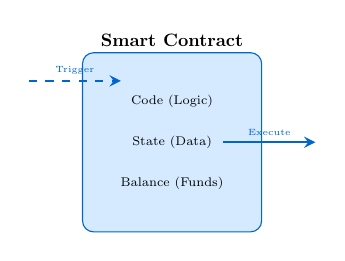
\begin{tikzpicture}[scale=0.65, transform shape]
    \node[rectangle, draw=dfblue, fill=dflightblue4, minimum width=3.5cm, minimum height=3.5cm, rounded corners] (contract) at (0,0) {};
    \node[above] at (contract.north) {\textbf{Smart Contract}};
    \node[align=center, font=\scriptsize] at (0,0.8) {Code (Logic)};
    \node[align=center, font=\scriptsize] at (0,0) {State (Data)};
    \node[align=center, font=\scriptsize] at (0,-0.8) {Balance (Funds)};

    \draw[arrow, dashed] (-2.8,1.2) -- (-1,1.2) node[midway, above, font=\tiny] {Trigger};
    \draw[arrow] (1,0) -- (2.8,0) node[midway, above, font=\tiny] {Execute};
\end{tikzpicture}

\vspace{0.3cm}
\begin{alertblock}{Key Insight}
DeFi replaces financial intermediaries with auditable code.
\end{alertblock}
\end{column}
\end{columns}
\end{frame}

% =====================================================================
% SLIDE 4: PREREQUISITES - THE TRUST SPECTRUM
% =====================================================================
\begin{frame}{From Smart Contracts to DeFi}
\begin{center}
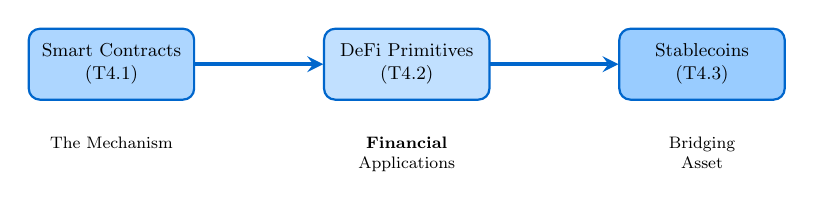
\begin{tikzpicture}[scale=0.75, transform shape]
    % Nodes
    \node[smartcontract, minimum width=2.8cm, minimum height=1.2cm] (sc) at (0,0) {Smart Contracts\\(T4.1)};
    \node[smartcontract, minimum width=2.8cm, minimum height=1.2cm, fill=dflightblue3] (defi) at (5,0) {DeFi Primitives\\(T4.2)};
    \node[smartcontract, minimum width=2.8cm, minimum height=1.2cm, fill=dflightblue] (stable) at (10,0) {Stablecoins\\(T4.3)};

    % Arrows
    \draw[arrow, line width=1.5pt] (sc) -- (defi);
    \draw[arrow, line width=1.5pt] (defi) -- (stable);

    % Labels below
    \node[below=0.5cm of sc, text width=2.5cm, align=center, font=\footnotesize] {The Mechanism};
    \node[below=0.5cm of defi, text width=2.5cm, align=center, font=\footnotesize] {\textbf{Financial}\\Applications};
    \node[below=0.5cm of stable, text width=2.5cm, align=center, font=\footnotesize] {Bridging\\Asset};
\end{tikzpicture}
\end{center}

\vspace{0.3cm}
\textbf{The Building Block Progression:}
\begin{enumerate}
    \item \textbf{T4.1}: Smart contracts provide the \textit{mechanism} for trustless execution
    \item \textbf{T4.2}: DeFi primitives build \textit{financial applications} on that mechanism
    \item \textbf{T4.3}: Stablecoins provide the \textit{stable value unit} for DeFi to function
\end{enumerate}

\vspace{0.2cm}
\begin{block}{Today's Focus}
How do we build trading, lending, and yield generation using only smart contracts?
\end{block}
\end{frame}

% =====================================================================
% SLIDE 5: WHAT IS DEFI?
% =====================================================================
\begin{frame}{What is DeFi?}
\begin{columns}[T]
\begin{column}{0.55\textwidth}
\begin{block}{Definition}
\textbf{Decentralized Finance (DeFi)} refers to financial services built on public blockchains that operate without traditional intermediaries.

\vspace{0.2cm}
\textit{Concrete Example:} Imagine borrowing money directly from strangers worldwide with no bank in the middle. The smart contract automatically manages collateral, interest rates, and repayment.
\end{block}

\vspace{0.3cm}
\textbf{Core Principles:}
\begin{itemize}
    \item \textbf{Permissionless}: Anyone can participate
    \item \textbf{Non-custodial}: Users control their assets
    \item \textbf{Transparent}: All code and transactions public
    \item \textbf{Composable}: Protocols can be combined
\end{itemize}
\end{column}

\begin{column}{0.42\textwidth}
\textbf{DeFi Ecosystem (2024):}
\begin{itemize}
    \item Total Value Locked (TVL = Total Value Locked = money deposited in DeFi protocols): \$50B+
    \item[]{\footnotesize \textcolor{dfgray}{\textit{That's more than the GDP of some countries!}}}
    \item Daily trading volume: \$2B+
    \item Active protocols: 500+
    \item Supported chains: 50+
\end{itemize}

\vspace{0.3cm}
\textbf{Major Categories:}
\begin{itemize}
    \item Decentralized Exchanges
    \item Lending Protocols
    \item Derivatives
    \item Yield Aggregators
\end{itemize}
\end{column}
\end{columns}
\end{frame}

% =====================================================================
% SLIDE 6: DEFI VS TRADITIONAL FINANCE
% =====================================================================
\begin{frame}{DeFi vs. Traditional Finance}
\begin{center}
\begin{tabular}{p{3cm}|p{5cm}|p{5cm}}
\toprule
\textbf{Feature} & \textbf{Traditional Finance} & \textbf{DeFi} \\
\midrule
Access & KYC (Know Your Customer = proving you are who you say you are), credit checks & Wallet address only \\
Hours & Business hours, T+2 settlement (2 days to finalize) & 24/7/365, instant \\
Custody & Institutions hold assets & User self-custody \\
Transparency & Private ledgers & Public blockchain \\
Innovation & Regulatory approval needed & Permissionless deployment \\
Risk & Counterparty, institution & Smart contract, oracle \\
\bottomrule
\end{tabular}
\end{center}

\vspace{0.3cm}
\begin{alertblock}{The Composability Advantage}
DeFi protocols are like ``money legos''---they can be combined in ways their creators never anticipated. A flash loan can be used in an arbitrage that spans 5 different protocols in a single transaction.
\end{alertblock}
\end{frame}

% =====================================================================
% SLIDE 7: THE DEFI STACK
% =====================================================================
\begin{frame}{The DeFi Stack}
\begin{center}
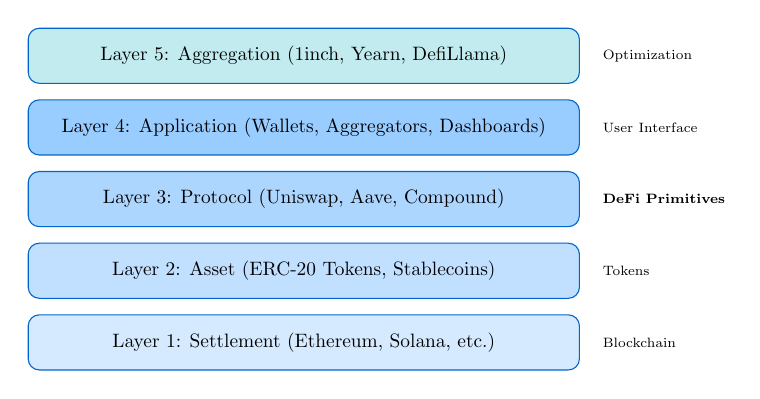
\begin{tikzpicture}[scale=0.7, transform shape]
    % Stack layers
    \node[rectangle, draw=dfblue, fill=dflightblue4, minimum width=10cm, minimum height=1cm, rounded corners] (l1) at (0,0) {Layer 1: Settlement (Ethereum, Solana, etc.)};

    \node[rectangle, draw=dfblue, fill=dflightblue3, minimum width=10cm, minimum height=1cm, rounded corners] (l2) at (0,1.3) {Layer 2: Asset (ERC-20 Tokens, Stablecoins)};

    \node[rectangle, draw=dfblue, fill=dflightblue2, minimum width=10cm, minimum height=1cm, rounded corners] (l3) at (0,2.6) {Layer 3: Protocol (Uniswap, Aave, Compound)};

    \node[rectangle, draw=dfblue, fill=dflightblue, minimum width=10cm, minimum height=1cm, rounded corners] (l4) at (0,3.9) {Layer 4: Application (Wallets, Aggregators, Dashboards)};

    \node[rectangle, draw=dfblue, fill=dfcyan!30, minimum width=10cm, minimum height=1cm, rounded corners] (l5) at (0,5.2) {Layer 5: Aggregation (1inch, Yearn, DefiLlama)};

    % Labels
    \node[right, font=\scriptsize] at (5.3,0) {Blockchain};
    \node[right, font=\scriptsize] at (5.3,1.3) {Tokens};
    \node[right, font=\scriptsize] at (5.3,2.6) {\textbf{DeFi Primitives}};
    \node[right, font=\scriptsize] at (5.3,3.9) {User Interface};
    \node[right, font=\scriptsize] at (5.3,5.2) {Optimization};
\end{tikzpicture}
\end{center}

\vspace{0.2cm}
\textbf{Today's Focus}: Layer 3 -- The core protocols that enable decentralized trading and lending
\end{frame}

% =====================================================================
% SLIDE 8: INTRODUCING AMMS
% =====================================================================
\begin{frame}{Automated Market Makers (AMMs)}
\begin{columns}[T]
\begin{column}{0.48\textwidth}
\textbf{Traditional Exchange:}
\begin{itemize}
    \item Order book with bids/asks (like an auction where buyers and sellers post their desired prices)
    \item Market makers provide liquidity
    \item Requires active management
    \item Centralized matching engine
\end{itemize}

\vspace{0.3cm}
\textbf{AMM Innovation:}
\begin{itemize}
    \item No order book needed
    \item Liquidity pools replace market makers
    \item Algorithmic pricing
    \item Anyone can provide liquidity
\end{itemize}
\end{column}

\begin{column}{0.48\textwidth}
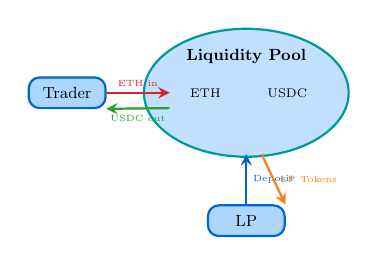
\begin{tikzpicture}[scale=0.65, transform shape]
    % Pool
    \node[pool, minimum width=4cm, minimum height=2.5cm] (pool) at (0,0) {};
    \node[font=\small\bfseries] at (0, 0.7) {Liquidity Pool};
    \node[font=\scriptsize] at (-0.8, 0) {ETH};
    \node[font=\scriptsize] at (0.8, 0) {USDC};

    % Trader
    \node[smartcontract, minimum width=1.5cm, minimum height=0.6cm] (trader) at (-3.5, 0) {Trader};

    % LP
    \node[smartcontract, minimum width=1.5cm, minimum height=0.6cm] (lp) at (0, -2.5) {LP};

    % Arrows
    \draw[arrow, dfred] (trader) -- (-1.5, 0) node[midway, above, font=\tiny] {ETH in};
    \draw[arrow, dfgreen] (-1.5, -0.3) -- (trader.south east) node[midway, below, font=\tiny] {USDC out};

    \draw[arrow, dfblue] (lp) -- (0, -1.2) node[midway, right, font=\tiny] {Deposit};
    \draw[arrow, dforange] (0.3, -1.2) -- (lp.north east) node[midway, right, font=\tiny] {LP Tokens};
\end{tikzpicture}
\end{column}
\end{columns}

\vspace{0.2cm}
\textbf{Key Protocols:}
\begin{itemize}
    \item \textbf{Uniswap}: Most popular AMM, simple constant product formula
    \item \textbf{SushiSwap}: Uniswap fork with community governance
    \item \textbf{Curve}: Optimized for stablecoin swaps (low slippage)
    \item \textbf{Balancer}: Multi-token pools with custom weights
\end{itemize}
\end{frame}

% =====================================================================
% SLIDE 9: FOLLOW THE MONEY WALKTHROUGH
% =====================================================================
\begin{frame}{Follow the Money: How AMMs Work (Step-by-Step)}
\begin{block}{Scenario: You Want to Swap 1 ETH for USDC}
\textbf{Initial Pool State:}
\begin{itemize}
    \item Pool has: 100 ETH + 300,000 USDC
    \item Current price: 1 ETH = 3,000 USDC
\end{itemize}
\end{block}

\textbf{Step 1:} You deposit 1 ETH into the pool
\begin{itemize}
    \item Pool now has: \textcolor{dfblue}{101 ETH} + 300,000 USDC
\end{itemize}

\textbf{Step 2:} The pool removes USDC to keep the product constant
\begin{itemize}
    \item Before: $100 \times 300,000 = 30,000,000$
    \item After: $101 \times ? = 30,000,000$
    \item Solve: $? = 30,000,000 \div 101 = 297,030$ USDC
\end{itemize}

\textbf{Step 3:} You receive the difference
\begin{itemize}
    \item USDC removed: $300,000 - 297,030 = \textcolor{dfgreen}{2,970 USDC}$
    \item You get slightly less than 3,000 USDC due to price impact!
\end{itemize}
\end{frame}

% =====================================================================
% SLIDE 10: THE CONSTANT PRODUCT FORMULA
% =====================================================================
\begin{frame}{The Constant Product Formula: $x \cdot y = k$}
\begin{columns}[T]
\begin{column}{0.45\textwidth}
\begin{block}{The Core Equation}
\[
x \cdot y = k
\]
\begin{itemize}
    \item $x$ = Token A reserves
    \item $y$ = Token B reserves
    \item $k$ = Constant (invariant)
\end{itemize}
\end{block}

\vspace{0.2cm}
\textbf{Price Determination:}
\[
\text{Price of A in B} = \frac{y}{x}
\]

\textbf{After swap of $\Delta x$:}
\[
\Delta y = y - \frac{k}{x + \Delta x}
\]
\end{column}

\begin{column}{0.52\textwidth}
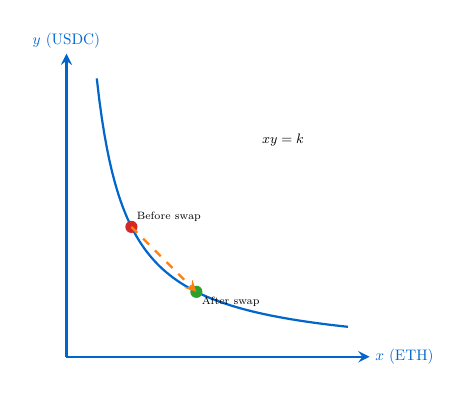
\begin{tikzpicture}[scale=0.55, transform shape]
    % Axes
    \draw[arrow] (0,0) -- (7,0) node[right] {$x$ (ETH)};
    \draw[arrow] (0,0) -- (0,7) node[above] {$y$ (USDC)};

    % Curve xy = k
    \draw[thick, dfblue, domain=0.7:6.5, samples=100] plot (\x, {4.5/\x});

    % Points
    \fill[dfred] (1.5, 3) circle (4pt);
    \node[above right, font=\scriptsize] at (1.5, 3) {Before swap};

    \fill[dfgreen] (3, 1.5) circle (4pt);
    \node[below right, font=\scriptsize] at (3, 1.5) {After swap};

    % Trade arrow
    \draw[arrow, dforange, thick, dashed] (1.5, 3) -- (3, 1.5);

    % Label
    \node[font=\small] at (5, 5) {$xy = k$};
\end{tikzpicture}
\end{column}
\end{columns}

\vspace{0.2cm}
\begin{alertblock}{Price Impact}
Larger trades move further along the curve, resulting in worse prices. This is called \textbf{slippage} or \textbf{price impact}.
\end{alertblock}
\end{frame}

% =====================================================================
% SLIDE 11: AMM NUMERICAL EXAMPLE
% =====================================================================
\begin{frame}{AMM Numerical Example}
\begin{block}{Initial Pool State}
\begin{itemize}
    \item 100 ETH + 300,000 USDC
    \item $k = 100 \times 300,000 = 30,000,000$
    \item Price: 1 ETH = 3,000 USDC
\end{itemize}
\end{block}

\textbf{Trader swaps 10 ETH for USDC:}
\begin{align*}
\text{New ETH reserves:} \quad x' &= 100 + 10 = 110 \\
\text{New USDC reserves:} \quad y' &= \frac{30,000,000}{110} = 272,727.27 \\
\text{USDC received:} \quad \Delta y &= 300,000 - 272,727.27 = 27,272.73
\end{align*}

\begin{alertblock}{Price Impact Analysis}
\begin{itemize}
    \item Expected (no impact): $10 \times 3,000 = 30,000$ USDC
    \item Actual received: 27,272.73 USDC
    \item Slippage: $\frac{30,000 - 27,272.73}{30,000} = 9.09\%$
    \item New price: $\frac{272,727.27}{110} = 2,479.34$ USDC/ETH
\end{itemize}
\end{alertblock}
\end{frame}

% =====================================================================
% SLIDE 12: WHY SLIPPAGE GROWS NON-LINEARLY
% =====================================================================
\begin{frame}{Why Larger Trades Have More Slippage}
\begin{columns}[T]
\begin{column}{0.48\textwidth}
\textbf{Trade Size vs. Slippage:}
\begin{center}
\begin{tabular}{ccc}
\toprule
\textbf{Trade} & \textbf{Slippage} & \textbf{Cost} \\
\midrule
1 ETH & 0.99\% & \$30 \\
5 ETH & 4.76\% & \$714 \\
10 ETH & 9.09\% & \$2,727 \\
20 ETH & 16.67\% & \$10,000 \\
50 ETH & 33.33\% & \$50,000 \\
\bottomrule
\end{tabular}
\end{center}

\vspace{0.2cm}
{\footnotesize \textcolor{dfgray}{\textit{What This Costs You: Dollar amounts lost compared to no slippage (at \$3,000/ETH)}}}

\vspace{0.3cm}
\textbf{Key Insight:}
Slippage grows \textit{non-linearly} because larger trades shift the reserve ratio more dramatically.
\end{column}

\begin{column}{0.48\textwidth}
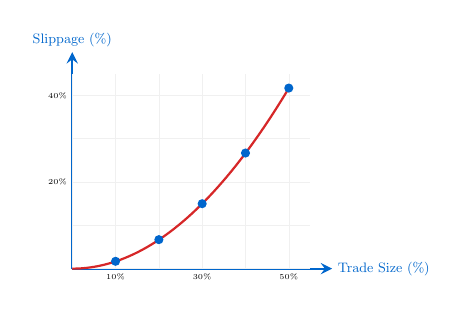
\begin{tikzpicture}[scale=0.55, transform shape]
    % Axes
    \draw[arrow] (0,0) -- (6,0) node[right, font=\small] {Trade Size (\%)};
    \draw[arrow] (0,0) -- (0,5) node[above, font=\small] {Slippage (\%)};

    % Grid
    \draw[very thin, lightgray] (0,0) grid (5.5,4.5);

    % Slippage curve (approximation)
    \draw[thick, dfred, domain=0:5, samples=50] plot (\x, {\x*\x/6});

    % Points
    \fill[dfblue] (1, 0.17) circle (3pt);
    \fill[dfblue] (2, 0.67) circle (3pt);
    \fill[dfblue] (3, 1.5) circle (3pt);
    \fill[dfblue] (4, 2.67) circle (3pt);
    \fill[dfblue] (5, 4.17) circle (3pt);

    % Labels
    \node[below, font=\tiny] at (1,0) {10\%};
    \node[below, font=\tiny] at (3,0) {30\%};
    \node[below, font=\tiny] at (5,0) {50\%};
    \node[left, font=\tiny] at (0,2) {20\%};
    \node[left, font=\tiny] at (0,4) {40\%};
\end{tikzpicture}
\end{column}
\end{columns}

\vspace{0.3cm}
\begin{block}{Practical Implication}
Deep liquidity pools (high TVL) have less slippage for the same trade size. Always check price impact before executing large trades.
\end{block}
\end{frame}

% =====================================================================
% SLIDE 13: LIQUIDITY POOL MECHANICS
% =====================================================================
\begin{frame}{Liquidity Pool Mechanics}
\begin{center}
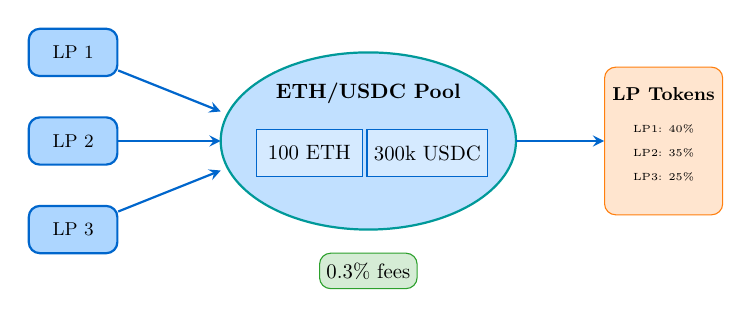
\begin{tikzpicture}[scale=0.75, transform shape]
    % Pool
    \node[pool, minimum width=5cm, minimum height=3cm, fill=dflightblue3] (pool) at (0,0) {};
    \node[font=\bfseries] at (0, 0.8) {ETH/USDC Pool};

    % Reserves
    \node[rectangle, draw=dfblue, fill=dflightblue4, minimum width=1.8cm, minimum height=0.8cm] at (-1, -0.2) {100 ETH};
    \node[rectangle, draw=dfblue, fill=dflightblue4, minimum width=1.8cm, minimum height=0.8cm] at (1, -0.2) {300k USDC};

    % LPs
    \node[smartcontract, minimum width=1.5cm] (lp1) at (-5, 1.5) {LP 1};
    \node[smartcontract, minimum width=1.5cm] (lp2) at (-5, 0) {LP 2};
    \node[smartcontract, minimum width=1.5cm] (lp3) at (-5, -1.5) {LP 3};

    % LP tokens
    \node[rectangle, draw=dforange, fill=dforange!20, minimum width=2cm, minimum height=2.5cm, rounded corners] (lptokens) at (5, 0) {};
    \node[font=\small\bfseries] at (5, 0.8) {LP Tokens};
    \node[font=\tiny] at (5, 0.2) {LP1: 40\%};
    \node[font=\tiny] at (5, -0.2) {LP2: 35\%};
    \node[font=\tiny] at (5, -0.6) {LP3: 25\%};

    % Arrows
    \draw[arrow] (lp1) -- (-2.5, 0.5);
    \draw[arrow] (lp2) -- (-2.5, 0);
    \draw[arrow] (lp3) -- (-2.5, -0.5);

    \draw[arrow] (2.5, 0) -- (lptokens);

    % Fees
    \node[rectangle, draw=dfgreen, fill=dfgreen!20, minimum width=1.5cm, minimum height=0.6cm, rounded corners] at (0, -2.2) {0.3\% fees};
\end{tikzpicture}
\end{center}

\textbf{LP Token Mechanics:}
\begin{itemize}
    \item LP tokens represent proportional claim on pool reserves
    \item Fees accumulate in pool, increasing LP token value
    \item Withdrawal returns proportional share of \textit{current} reserves
\end{itemize}
\end{frame}

% =====================================================================
% SLIDE 14: LP TOKENS DEEP DIVE
% =====================================================================
\begin{frame}{LP Tokens: Ownership and Fee Accrual}
\begin{columns}[T]
\begin{column}{0.48\textwidth}
\textbf{How LP Tokens Work:}
\begin{enumerate}
    \item Deposit both tokens in equal value
    \item Receive LP tokens proportional to contribution
    \item First deposit: $\text{LP} = \sqrt{x \cdot y}$
    \item Later deposits: proportional to pool share
\end{enumerate}

\vspace{0.3cm}
\textbf{Example:}
\begin{itemize}
    \item Pool: 1,000 total LP tokens
    \item You hold: 100 LP tokens (10\%)
    \item You own 10\% of all reserves
    \item Plus 10\% of accumulated fees
\end{itemize}
\end{column}

\begin{column}{0.48\textwidth}
\textbf{Fee Accrual Mechanism:}
\begin{itemize}
    \item Trading fees stay in the pool
    \item Reserves grow with each trade
    \item LP token supply unchanged
    \item Each LP token worth more over time
\end{itemize}

\vspace{0.3cm}
\begin{alertblock}{Key Point}
Fees aren't distributed separately---they accumulate in the pool. You receive your share when you withdraw by burning LP tokens.
\end{alertblock}
\end{column}
\end{columns}
\end{frame}

% =====================================================================
% SLIDE 15: IMPERMANENT LOSS EXPLAINED
% =====================================================================
\begin{frame}{Impermanent Loss Explained}
\begin{block}{Definition}
\textbf{Impermanent Loss (IL)} is the difference between holding assets in a liquidity pool vs. simply holding them in your wallet.
\end{block}

\textbf{Why it happens:}
\begin{enumerate}
    \item You deposit equal value: 1 ETH (\$3,000) + 3,000 USDC
    \item ETH price doubles to \$6,000
    \item Arbitrageurs rebalance the pool
    \item Your LP position: 0.707 ETH + 4,243 USDC = \$8,485
    \item If you had just held: 1 ETH + 3,000 USDC = \$9,000
    \item \textbf{Impermanent Loss: \$515 (5.72\%)}
\end{enumerate}

\vspace{0.2cm}
\begin{alertblock}{Key Insight}
Loss is ``impermanent'' because if prices return to original levels, the loss disappears. It becomes \textit{permanent} when you withdraw at different prices.
\end{alertblock}
\end{frame}

% =====================================================================
% SLIDE 16: IMPERMANENT LOSS FORMULA
% =====================================================================
\begin{frame}{Impermanent Loss Formula and Visualization}
\begin{columns}[T]
\begin{column}{0.45\textwidth}
\textbf{IL Formula:}
\[
IL = \frac{2\sqrt{r}}{1+r} - 1
\]
where $r = \frac{P_1}{P_0}$ (price ratio)

\vspace{0.3cm}
\begin{tabular}{cc}
\toprule
\textbf{Price Change} & \textbf{IL} \\
\midrule
1.25x (25\% up) & 0.6\% \\
1.50x (50\% up) & 2.0\% \\
2x (100\% up) & 5.7\% \\
3x (200\% up) & 13.4\% \\
4x (300\% up) & 20.0\% \\
5x (400\% up) & 25.5\% \\
\bottomrule
\end{tabular}
\end{column}

\begin{column}{0.52\textwidth}
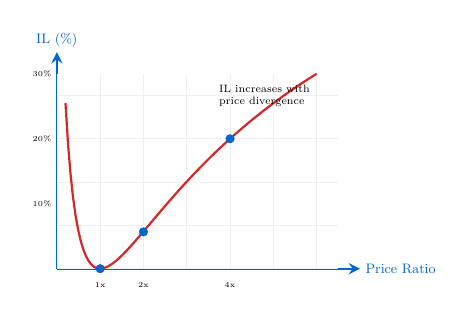
\begin{tikzpicture}[scale=0.55, transform shape]
    % Axes
    \draw[arrow] (0,0) -- (7,0) node[right, font=\small] {Price Ratio};
    \draw[arrow] (0,0) -- (0,5) node[above, font=\small] {IL (\%)};

    % Grid
    \draw[very thin, lightgray] (0,0) grid (6.5,4.5);

    % IL curve
    \draw[thick, dfred, domain=0.2:6, samples=100] plot (\x, {(1 - 2*sqrt(\x)/(1+\x))*15});

    % Points
    \fill[dfblue] (1, 0) circle (3pt);
    \node[below, font=\tiny] at (1, -0.2) {1x};

    \fill[dfblue] (2, 0.85) circle (3pt);
    \node[below, font=\tiny] at (2, -0.2) {2x};

    \fill[dfblue] (4, 3) circle (3pt);
    \node[below, font=\tiny] at (4, -0.2) {4x};

    % Y-axis labels
    \node[left, font=\tiny] at (0, 1.5) {10\%};
    \node[left, font=\tiny] at (0, 3) {20\%};
    \node[left, font=\tiny] at (0, 4.5) {30\%};

    % Annotation
    \node[font=\scriptsize, text width=2.5cm] at (5, 4) {IL increases with price divergence};
\end{tikzpicture}
\end{column}
\end{columns}

\vspace{0.2cm}
\textbf{Mitigating IL:}
\begin{itemize}
    \item Provide liquidity to correlated pairs (stablecoin-stablecoin)
    \item Choose pools with high trading volume (fees offset IL)
    \item Use concentrated liquidity (Uniswap V3)
\end{itemize}
\end{frame}

% =====================================================================
% SLIDE 17: IL WORKED EXAMPLE
% =====================================================================
\begin{frame}{Impermanent Loss: Worked Example}
\begin{columns}[T]
\begin{column}{0.48\textwidth}
\textbf{Initial State:}
\begin{itemize}
    \item Deposit: 1 ETH + 2,000 USDC
    \item Initial value: \$4,000
    \item ETH price: \$2,000
\end{itemize}

\vspace{0.3cm}
\textbf{Price Change:}
\begin{itemize}
    \item New ETH price: \$4,000 (2x)
    \item Price ratio $r = 2$
\end{itemize}

\vspace{0.3cm}
\textbf{If Just Holding:}
\begin{itemize}
    \item 1 ETH $\times$ \$4,000 = \$4,000
    \item 2,000 USDC = \$2,000
    \item Total: \textbf{\$6,000}
\end{itemize}
\end{column}

\begin{column}{0.48\textwidth}
\textbf{In the Pool:}
\begin{itemize}
    \item Pool rebalances via arbitrage
    \item New position: 0.707 ETH + 2,828 USDC
    \item Value: $0.707 \times 4000 + 2828$
    \item Total: \textbf{\$5,657}
\end{itemize}

\vspace{0.3cm}
\textbf{Impermanent Loss:}
\[
IL = \frac{2\sqrt{2}}{1+2} - 1 = -5.72\%
\]
\[
\text{Loss} = 6000 - 5657 = \$343
\]

\vspace{0.2cm}
\begin{alertblock}{Break-Even}
Trading fees must exceed \$343 to be profitable!
\end{alertblock}
\end{column}
\end{columns}
\end{frame}

% =====================================================================
% SLIDE 18: ARBITRAGE IN AMMS
% =====================================================================
\begin{frame}{The Role of Arbitrage in AMMs}
\begin{columns}[T]
\begin{column}{0.48\textwidth}
\textbf{How Price Discovery Works:}
\begin{enumerate}
    \item External price changes (e.g., on Binance)
    \item AMM price diverges from market
    \item Arbitrageurs profit by trading the difference
    \item AMM price converges to market price
\end{enumerate}

\vspace{0.3cm}
\textbf{Example:}
\begin{itemize}
    \item AMM price: 1 ETH = \$2,000
    \item Binance price: 1 ETH = \$2,100
    \item Arbitrageur buys cheap on AMM
    \item Sells expensive on Binance
    \item AMM price increases toward \$2,100
\end{itemize}
\end{column}

\begin{column}{0.48\textwidth}
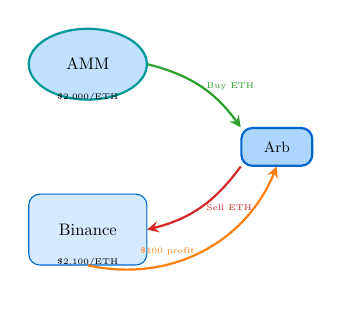
\begin{tikzpicture}[scale=0.6, transform shape]
    % AMM
    \node[pool, minimum width=2.5cm, minimum height=1.5cm] (amm) at (0, 2) {AMM};
    \node[font=\tiny] at (0, 1.3) {\$2,000/ETH};

    % CEX
    \node[rectangle, draw=dfblue, fill=dflightblue4, minimum width=2.5cm, minimum height=1.5cm, rounded corners] (cex) at (0, -1.5) {Binance};
    \node[font=\tiny] at (0, -2.2) {\$2,100/ETH};

    % Arbitrageur
    \node[smartcontract, minimum width=1.5cm] (arb) at (4, 0.25) {Arb};

    % Arrows
    \draw[arrow, dfgreen] (amm.east) to[bend left=20] node[midway, right, font=\tiny] {Buy ETH} (arb.north west);
    \draw[arrow, dfred] (arb.south west) to[bend left=20] node[midway, right, font=\tiny] {Sell ETH} (cex.east);
    \draw[arrow, dforange] (cex.south) to[bend right=40] node[midway, left, font=\tiny] {\$100 profit} (arb.south);
\end{tikzpicture}

\vspace{0.3cm}
\begin{alertblock}{Key Insight}
Arbitrage is the mechanism that keeps AMM prices aligned with external markets---without oracles!
\end{alertblock}
\end{column}
\end{columns}
\end{frame}

% =====================================================================
% SLIDE 19: DEFI LENDING OVERVIEW
% =====================================================================
\begin{frame}{DeFi Lending: How It Works}
\begin{center}
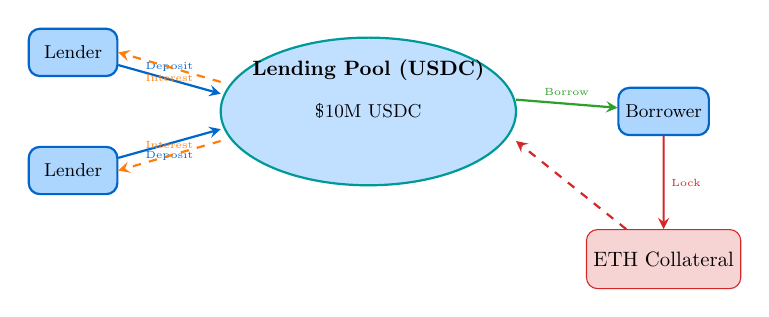
\begin{tikzpicture}[scale=0.75, transform shape]
    % Lending Pool
    \node[pool, minimum width=5cm, minimum height=2.5cm] (pool) at (0,0) {};
    \node[font=\bfseries] at (0, 0.7) {Lending Pool (USDC)};
    \node[font=\small] at (0, 0) {\$10M USDC};

    % Lenders
    \node[smartcontract, minimum width=1.5cm] (lend1) at (-5, 1) {Lender};
    \node[smartcontract, minimum width=1.5cm] (lend2) at (-5, -1) {Lender};

    % Borrowers
    \node[smartcontract, minimum width=1.5cm] (borrow) at (5, 0) {Borrower};

    % Collateral box
    \node[rectangle, draw=dfred, fill=dfred!20, minimum width=2cm, minimum height=1cm, rounded corners] (collat) at (5, -2.5) {ETH Collateral};

    % Arrows
    \draw[arrow, dfblue] (lend1) -- (-2.5, 0.3) node[midway, above, font=\tiny] {Deposit};
    \draw[arrow, dfblue] (lend2) -- (-2.5, -0.3) node[midway, below, font=\tiny] {Deposit};

    \draw[arrow, dfgreen] (2.5, 0.2) -- (borrow) node[midway, above, font=\tiny] {Borrow};
    \draw[arrow, dfred] (borrow) -- (collat) node[midway, right, font=\tiny] {Lock};
    \draw[arrow, dfred, dashed] (collat) -- (2.5, -0.5);

    % Interest arrows
    \draw[arrow, dforange, dashed] (-2.5, 0.5) -- (lend1.east) node[midway, below, font=\tiny] {Interest};
    \draw[arrow, dforange, dashed] (-2.5, -0.5) -- (lend2.east) node[midway, above, font=\tiny] {Interest};
\end{tikzpicture}
\end{center}

\textbf{Key Mechanics:}
\begin{itemize}
    \item \textbf{Over-collateralization}: Borrow \$1,000 requires \$1,500+ collateral
    \item \textbf{Algorithmic rates}: Interest adjusts with utilization
    \item \textbf{Liquidation}: If collateral falls below threshold, anyone can liquidate
\end{itemize}
\end{frame}

% =====================================================================
% SLIDE 20: ALGORITHMIC INTEREST RATES
% =====================================================================
\begin{frame}{Algorithmic Interest Rates}
\begin{columns}[T]
\begin{column}{0.45\textwidth}
\textbf{Utilization Rate:}
\[
U = \frac{\text{Borrowed}}{\text{Supplied}}
\]

\textbf{Borrow Rate (kinked model):}
\[
R_{\text{borrow}} =
\begin{cases}
R_0 + U \cdot R_{\text{slope1}} & U < U_{\text{opt}} \\
R_0 + U_{\text{opt}} \cdot R_1 + \\
\quad (U - U_{\text{opt}}) \cdot R_2 & U \geq U_{\text{opt}}
\end{cases}
\]

\textbf{Supply Rate:}
\[
R_{\text{supply}} = R_{\text{borrow}} \times U \times (1 - \text{fee})
\]
\end{column}

\begin{column}{0.52\textwidth}
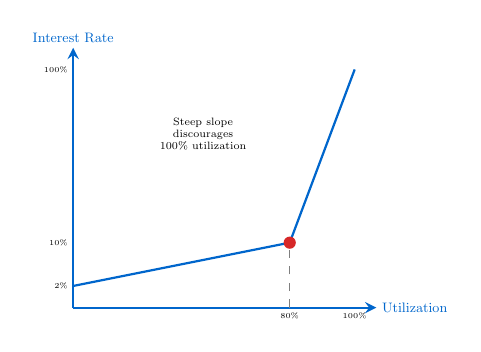
\begin{tikzpicture}[scale=0.55, transform shape]
    % Axes
    \draw[arrow] (0,0) -- (7,0) node[right, font=\small] {Utilization};
    \draw[arrow] (0,0) -- (0,6) node[above, font=\small] {Interest Rate};

    % Kinked curve
    \draw[thick, dfblue] (0, 0.5) -- (5, 1.5);
    \draw[thick, dfblue] (5, 1.5) -- (6.5, 5.5);

    % Optimal point
    \draw[dashed, dfgray] (5, 0) -- (5, 1.5);
    \fill[dfred] (5, 1.5) circle (4pt);

    % Labels
    \node[below, font=\tiny] at (5, 0) {80\%};
    \node[below, font=\tiny] at (6.5, 0) {100\%};
    \node[left, font=\tiny] at (0, 0.5) {2\%};
    \node[left, font=\tiny] at (0, 1.5) {10\%};
    \node[left, font=\tiny] at (0, 5.5) {100\%};

    % Annotation
    \node[font=\scriptsize, text width=2cm, align=center] at (3, 4) {Steep slope\\discourages\\100\% utilization};
\end{tikzpicture}
\end{column}
\end{columns}

\vspace{0.2cm}
\textbf{Key Protocols:} Aave, Compound, MakerDAO
\end{frame}

% =====================================================================
% SLIDE 21: LENDING EXAMPLE
% =====================================================================
\begin{frame}{DeFi Lending: Worked Example}
\begin{columns}[T]
\begin{column}{0.48\textwidth}
\textbf{Scenario:}
\begin{itemize}
    \item You have 10 ETH worth \$30,000
    \item Need \$15,000 USDC liquidity
    \item Don't want to sell your ETH
\end{itemize}

\vspace{0.3cm}
\textbf{DeFi Solution (Aave):}
\begin{enumerate}
    \item Deposit 10 ETH as collateral
    \item Borrow up to 75\% LTV = \$22,500
    \item You borrow \$15,000 USDC
    \item Pay 5\% APR interest
\end{enumerate}
\end{column}

\begin{column}{0.48\textwidth}
\textbf{Position Metrics:}
\begin{itemize}
    \item Collateral: \$30,000 (10 ETH)
    \item Debt: \$15,000 (USDC)
    \item Health Factor: $\frac{30000 \times 0.825}{15000} = 1.65$
    \item Liquidation at: HF $< 1.0$
\end{itemize}

\vspace{0.3cm}
\begin{alertblock}{Liquidation Risk}
If ETH drops 40\% to \$1,800:
\begin{itemize}
    \item New collateral: \$18,000
    \item Health Factor: $\frac{18000 \times 0.825}{15000} = 0.99$
    \item Position liquidated!
\end{itemize}
\end{alertblock}
\end{column}
\end{columns}
\end{frame}

% =====================================================================
% SLIDE 22: FLASH LOANS
% =====================================================================
\begin{frame}{Flash Loans: Innovation or Attack Vector?}
\begin{block}{Definition}
A \textbf{flash loan} is an uncollateralized loan that must be borrowed and repaid within a single transaction.
\end{block}

\begin{center}
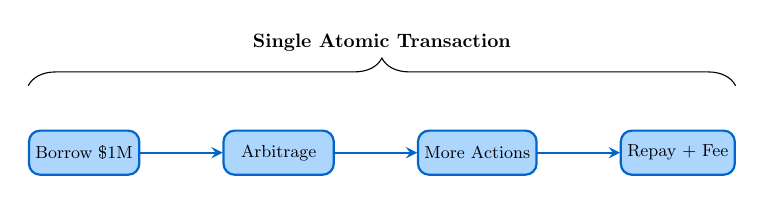
\begin{tikzpicture}[scale=0.7, transform shape, node distance=1.5cm]
    \node[smartcontract] (borrow) {Borrow \$1M};
    \node[smartcontract, right=of borrow] (use1) {Arbitrage};
    \node[smartcontract, right=of use1] (use2) {More Actions};
    \node[smartcontract, right=of use2] (repay) {Repay + Fee};

    \draw[arrow] (borrow) -- (use1);
    \draw[arrow] (use1) -- (use2);
    \draw[arrow] (use2) -- (repay);

    % Single transaction bracket
    \draw[decorate, decoration={brace, amplitude=10pt}]
        ([yshift=0.8cm]borrow.north west) -- ([yshift=0.8cm]repay.north east)
        node[midway, above=0.5cm] {\textbf{Single Atomic Transaction}};
\end{tikzpicture}
\end{center}

\textbf{Legitimate Uses:} Arbitrage, collateral swaps, self-liquidation

\textbf{Attack Uses:} Oracle manipulation, governance attacks, protocol exploits

\begin{alertblock}{The Double-Edged Sword}
Flash loans democratize access to capital but have enabled over \$500M in DeFi exploits.
\end{alertblock}
\end{frame}

% =====================================================================
% SLIDE 23: COMPOSABILITY - MONEY LEGOS
% =====================================================================
\begin{frame}{Composability: The ``Money Legos'' Concept}
\begin{columns}[T]
\begin{column}{0.48\textwidth}
\textbf{What is Composability?}
\begin{itemize}
    \item Protocols can call other protocols
    \item Build complex strategies from simple parts
    \item No permission needed to integrate
    \item Innovation without coordination
\end{itemize}

\vspace{0.3cm}
\textbf{Example Stack:}
\begin{enumerate}
    \item Deposit ETH into Aave
    \item Receive aETH (interest-bearing)
    \item Deposit aETH into Uniswap
    \item Earn trading fees + lending interest
\end{enumerate}
\end{column}

\begin{column}{0.48\textwidth}
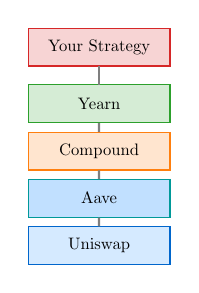
\begin{tikzpicture}[scale=0.6, transform shape]
    % Lego blocks
    \node[rectangle, draw=dfblue, fill=dflightblue4, minimum width=3cm, minimum height=0.8cm] (l1) at (0,0) {Uniswap};
    \node[rectangle, draw=dfteal, fill=dflightblue3, minimum width=3cm, minimum height=0.8cm] (l2) at (0,1) {Aave};
    \node[rectangle, draw=dforange, fill=dforange!20, minimum width=3cm, minimum height=0.8cm] (l3) at (0,2) {Compound};
    \node[rectangle, draw=dfgreen, fill=dfgreen!20, minimum width=3cm, minimum height=0.8cm] (l4) at (0,3) {Yearn};

    % Your strategy
    \node[rectangle, draw=dfred, fill=dfred!20, minimum width=3cm, minimum height=0.8cm] (user) at (0,4.2) {Your Strategy};

    % Connecting lines
    \draw[thick, dfgray] (l1) -- (l2);
    \draw[thick, dfgray] (l2) -- (l3);
    \draw[thick, dfgray] (l3) -- (l4);
    \draw[thick, dfgray] (l4) -- (user);
\end{tikzpicture}

\vspace{0.3cm}
\begin{alertblock}{Risk Compounds Too}
Composability creates \textit{systemic risk}---a bug in one protocol can cascade through the stack.
\end{alertblock}
\end{column}
\end{columns}
\end{frame}

% =====================================================================
% SLIDE 24: TVL AND DEFI METRICS
% =====================================================================
\begin{frame}{Understanding DeFi Metrics}
\begin{columns}[T]
\begin{column}{0.48\textwidth}
\textbf{Total Value Locked (TVL):}
\begin{itemize}
    \item Total assets deposited in protocol
    \item Indicator of protocol usage
    \item ETH/USDC Pool with 1,000 ETH (\$2M) + 2M USDC = \$4M TVL
\end{itemize}

\vspace{0.3cm}
\textbf{Other Key Metrics:}
\begin{itemize}
    \item \textbf{Volume}: Daily trading volume
    \item \textbf{Fees}: Revenue generated
    \item \textbf{APY}: Annual percentage yield
    \item \textbf{Health Factor}: Lending safety
\end{itemize}
\end{column}

\begin{column}{0.48\textwidth}
\textbf{Top DeFi Protocols (2024):}
\begin{center}
\begin{tabular}{lc}
\toprule
\textbf{Protocol} & \textbf{TVL} \\
\midrule
Lido & \$20B+ \\
Aave & \$10B+ \\
MakerDAO & \$8B+ \\
Uniswap & \$5B+ \\
Curve & \$2B+ \\
\bottomrule
\end{tabular}
\end{center}

\vspace{0.3cm}
\textbf{Why TVL Matters:}
\begin{itemize}
    \item Higher TVL = deeper liquidity
    \item Less slippage for traders
    \item More attractive to LPs
\end{itemize}
\end{column}
\end{columns}
\end{frame}

% =====================================================================
% SLIDE 25: DEFI RISKS
% =====================================================================
\begin{frame}{DeFi Risks: A Complete Picture}
\begin{columns}[T]
\begin{column}{0.48\textwidth}
\textbf{Smart Contract Risk:}
\begin{itemize}
    \item Bugs in code (The DAO: \$60M)
    \item Reentrancy attacks
    \item Logic errors
    \item Governance exploits
\end{itemize}

\vspace{0.3cm}
\textbf{Oracle Risk:}
\begin{itemize}
    \item Price manipulation
    \item Flash loan attacks
    \item Stale data
\end{itemize}
\end{column}

\begin{column}{0.48\textwidth}
\textbf{Economic Risk:}
\begin{itemize}
    \item Impermanent loss
    \item Liquidation cascades
    \item Bank runs on pools
\end{itemize}

\vspace{0.3cm}
\textbf{Systemic Risk:}
\begin{itemize}
    \item Protocol dependencies
    \item Stablecoin de-pegs
    \item Contagion effects
\end{itemize}

\vspace{0.2cm}
\begin{alertblock}{Key Insight}
DeFi doesn't eliminate risk---it transforms and redistributes it.
\end{alertblock}
\end{column}
\end{columns}
\end{frame}

% =====================================================================
% SLIDE 26: HANDS-ON EXERCISE INTRO
% =====================================================================
\begin{frame}{Hands-On Exercise: NB09 -- AMM Simulation}
\begin{center}
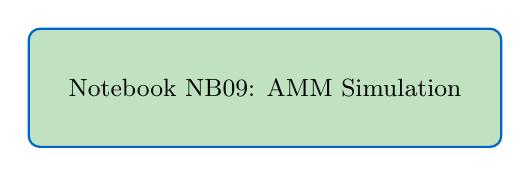
\begin{tikzpicture}
    \node[smartcontract, minimum width=6cm, minimum height=1.5cm, fill=dfgreen!30] {Notebook NB09: AMM Simulation};
\end{tikzpicture}
\end{center}

\vspace{0.3cm}
\textbf{What You Will Do:}
\begin{enumerate}
    \item \textbf{Create a Liquidity Pool}: Initialize with ETH and USDC reserves
    \item \textbf{Execute Swaps}: Trade tokens and observe price changes
    \item \textbf{Provide Liquidity}: Add liquidity and receive LP tokens
    \item \textbf{Measure Impermanent Loss}: Calculate IL for various price scenarios
    \item \textbf{Analyze Arbitrage}: See how arbitrage keeps prices aligned
\end{enumerate}

\vspace{0.3cm}
\textbf{Key Learning Outcomes:}
\begin{itemize}
    \item Practical understanding of $x \cdot y = k$
    \item Visualize slippage and price impact
    \item Experience the LP perspective
\end{itemize}
\end{frame}

% =====================================================================
% SLIDE 27: HANDS-ON EXERCISE PREVIEW
% =====================================================================
\begin{frame}[fragile]{NB09 Preview: Core AMM Functions}
\begin{lstlisting}[style=pythonstyle, basicstyle=\ttfamily\scriptsize]
class SimpleAMM:
    def __init__(self, reserve_x, reserve_y):
        self.x = reserve_x  # ETH
        self.y = reserve_y  # USDC
        self.k = reserve_x * reserve_y

    def get_spot_price(self):
        return self.y / self.x  # Price of X in terms of Y

    def swap_x_for_y(self, amount_x):
        # Apply constant product formula
        new_x = self.x + amount_x
        new_y = self.k / new_x
        amount_y_out = self.y - new_y
        self.x, self.y = new_x, new_y
        return amount_y_out

    def calculate_impermanent_loss(self, price_ratio):
        return 2 * sqrt(price_ratio) / (1 + price_ratio) - 1
\end{lstlisting}

\bottomnote{NB09 includes interactive visualizations of the bonding curve and IL}
\end{frame}

% =====================================================================
% SLIDE 28: DISCUSSION - DEFI IN PRACTICE
% =====================================================================
\begin{frame}{Discussion: DeFi in Practice}
\begin{block}{Case Study: The 2020 DeFi Summer}
\begin{itemize}
    \item TVL grew from \$1B to \$15B in 6 months
    \item Yield farming introduced liquidity mining
    \item Composability enabled rapid innovation
    \item Also: exploits, rug pulls, gas wars
\end{itemize}
\end{block}

\vspace{0.3cm}
\textbf{Discussion Questions:}
\begin{enumerate}
    \item Why did DeFi grow so rapidly in 2020?
    \item What are the barriers to mainstream DeFi adoption?
    \item How do DeFi risks compare to traditional finance risks?
    \item Can DeFi truly be ``decentralized'' if most users access it through centralized frontends?
\end{enumerate}
\end{frame}

% =====================================================================
% SLIDE 29: APPLICATION - REAL WORLD USE CASES
% =====================================================================
\begin{frame}{Real-World DeFi Applications}
\begin{columns}[T]
\begin{column}{0.48\textwidth}
\textbf{For Individuals:}
\begin{itemize}
    \item \textbf{Trading}: Swap tokens 24/7 without KYC
    \item \textbf{Lending}: Earn yield on idle assets
    \item \textbf{Borrowing}: Access liquidity without selling
    \item \textbf{Yield Farming}: Optimize returns across protocols
\end{itemize}

\vspace{0.3cm}
\textbf{For Institutions:}
\begin{itemize}
    \item Treasury management
    \item On-chain settlement
    \item Tokenized collateral
    \item Automated market making
\end{itemize}
\end{column}

\begin{column}{0.48\textwidth}
\textbf{Success Stories:}
\begin{itemize}
    \item Uniswap: \$1.5T+ cumulative volume
    \item Aave: \$10B+ in active loans
    \item Curve: \$100B+ stablecoin swaps
\end{itemize}

\vspace{0.3cm}
\textbf{Emerging Use Cases:}
\begin{itemize}
    \item Real-world asset lending
    \item Cross-border payments
    \item Institutional DeFi (permissioned pools)
    \item DeFi-TradFi bridges
\end{itemize}
\end{column}
\end{columns}
\end{frame}

% =====================================================================
% SLIDE 30: CRITICAL ANALYSIS
% =====================================================================
\begin{frame}{Critical Analysis: Is DeFi Really Decentralized?}
\begin{columns}[T]
\begin{column}{0.48\textwidth}
\textbf{Centralization Points:}
\begin{itemize}
    \item \textbf{Frontends}: Most users access via websites
    \item \textbf{Oracles}: Price feeds are critical dependencies
    \item \textbf{Governance}: Token holders control protocols
    \item \textbf{Infrastructure}: RPC providers, block builders
\end{itemize}

\vspace{0.3cm}
\textbf{The Ownership Question:}
\begin{itemize}
    \item Top 1\% often holds majority tokens
    \item VC funding creates concentrated ownership
    \item ``Decentralization theater''?
\end{itemize}
\end{column}

\begin{column}{0.48\textwidth}
\textbf{What IS Decentralized:}
\begin{itemize}
    \item Smart contract execution
    \item Permissionless access
    \item Transparent rules
    \item No single point of failure
\end{itemize}

\vspace{0.3cm}
\begin{block}{Nuanced View}
DeFi is more accurately ``disintermediated'' than ``decentralized.'' It removes certain intermediaries while creating new dependencies and power structures.
\end{block}
\end{column}
\end{columns}
\end{frame}

% =====================================================================
% SLIDE 31: FUTURE OF DEFI
% =====================================================================
\begin{frame}{The Future of DeFi}
\begin{columns}[T]
\begin{column}{0.48\textwidth}
\textbf{Technical Evolution:}
\begin{itemize}
    \item \textbf{Layer 2}: Lower fees, faster transactions
    \item \textbf{Cross-chain}: Unified liquidity across chains
    \item \textbf{Account Abstraction}: Better UX
    \item \textbf{Intent-based}: Express what, not how
\end{itemize}

\vspace{0.3cm}
\textbf{Market Evolution:}
\begin{itemize}
    \item Institutional adoption growing
    \item Regulatory clarity emerging
    \item TradFi-DeFi convergence
    \item Real-world asset integration
\end{itemize}
\end{column}

\begin{column}{0.48\textwidth}
\textbf{Key Challenges:}
\begin{itemize}
    \item Scalability limitations
    \item User experience complexity
    \item Regulatory uncertainty
    \item Smart contract risks
\end{itemize}

\vspace{0.3cm}
\begin{alertblock}{The Big Question}
Will DeFi remain a parallel financial system, or will it merge with traditional finance? The answer likely lies somewhere in between.
\end{alertblock}
\end{column}
\end{columns}
\end{frame}

% =====================================================================
% SLIDE 32: EXECUTIVE SUMMARY
% =====================================================================
\begin{frame}{Executive Summary}
\begin{block}{Core Concepts}
\begin{itemize}
    \item \textbf{AMMs} replace order books with liquidity pools and mathematical formulas ($x \cdot y = k$)
    \item \textbf{Liquidity providers} earn fees but face impermanent loss risk
    \item \textbf{DeFi lending} uses over-collateralization and algorithmic rates
    \item \textbf{Composability} enables innovation but creates systemic risk
    \item \textbf{Flash loans} democratize capital but enable attacks
\end{itemize}
\end{block}

\vspace{0.3cm}
\textbf{Key Equations:}
\begin{columns}[T]
\begin{column}{0.48\textwidth}
\begin{itemize}
    \item Constant Product: $x \cdot y = k$
    \item Spot Price: $P = \frac{y}{x}$
\end{itemize}
\end{column}
\begin{column}{0.48\textwidth}
\begin{itemize}
    \item Impermanent Loss: $IL = \frac{2\sqrt{r}}{1+r} - 1$
    \item Utilization: $U = \frac{\text{Borrowed}}{\text{Supplied}}$
\end{itemize}
\end{column}
\end{columns}
\end{frame}

% =====================================================================
% SLIDE 33: CONCEPT MAP
% =====================================================================
\begin{frame}{Concept Map: DeFi Primitives}
\begin{center}
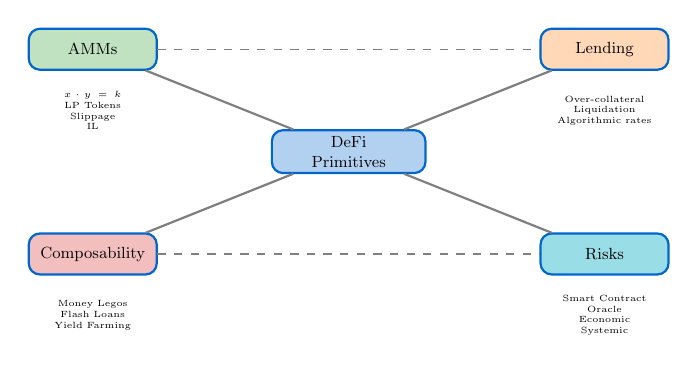
\begin{tikzpicture}[scale=0.65, transform shape]
    % Central node
    \node[smartcontract, minimum width=3cm, fill=dfblue!30] (center) at (0, 0) {DeFi\\Primitives};

    % Main branches
    \node[smartcontract, minimum width=2.5cm, fill=dfgreen!30] (amm) at (-5, 2) {AMMs};
    \node[smartcontract, minimum width=2.5cm, fill=dforange!30] (lending) at (5, 2) {Lending};
    \node[smartcontract, minimum width=2.5cm, fill=dfred!30] (compose) at (-5, -2) {Composability};
    \node[smartcontract, minimum width=2.5cm, fill=dfcyan!50] (risk) at (5, -2) {Risks};

    % AMM sub-nodes
    \node[font=\tiny, text width=2cm, align=center] at (-5, 0.8) {$x \cdot y = k$\\LP Tokens\\Slippage\\IL};

    % Lending sub-nodes
    \node[font=\tiny, text width=2cm, align=center] at (5, 0.8) {Over-collateral\\Liquidation\\Algorithmic rates};

    % Composability sub-nodes
    \node[font=\tiny, text width=2cm, align=center] at (-5, -3.2) {Money Legos\\Flash Loans\\Yield Farming};

    % Risk sub-nodes
    \node[font=\tiny, text width=2cm, align=center] at (5, -3.2) {Smart Contract\\Oracle\\Economic\\Systemic};

    % Connections
    \draw[thick, dfgray] (center) -- (amm);
    \draw[thick, dfgray] (center) -- (lending);
    \draw[thick, dfgray] (center) -- (compose);
    \draw[thick, dfgray] (center) -- (risk);

    % Cross connections
    \draw[dashed, dfgray] (amm) -- (lending);
    \draw[dashed, dfgray] (compose) -- (risk);
\end{tikzpicture}
\end{center}
\end{frame}

% =====================================================================
% SLIDE 34: KEY TERMS (PART 1)
% =====================================================================
\begin{frame}{Key Terms (Part 1)}
\begin{columns}[T]
\begin{column}{0.48\textwidth}
\textbf{AMM (Automated Market Maker):}\\
A protocol that uses algorithms to price assets instead of order books.

\vspace{0.3cm}
\textbf{Liquidity Pool:}\\
A smart contract holding reserves of two tokens for trading.

\vspace{0.3cm}
\textbf{LP Token:}\\
Token representing ownership share in a liquidity pool.

\vspace{0.3cm}
\textbf{Constant Product Formula:}\\
$x \cdot y = k$ --- the invariant that governs AMM pricing.
\end{column}

\begin{column}{0.48\textwidth}
\textbf{Slippage (Price Impact):}\\
The difference between expected and actual execution price.

\vspace{0.3cm}
\textbf{Impermanent Loss:}\\
Opportunity cost of providing liquidity vs. holding assets.

\vspace{0.3cm}
\textbf{TVL (Total Value Locked):}\\
Total assets deposited in a DeFi protocol.

\vspace{0.3cm}
\textbf{Utilization Rate:}\\
Percentage of supplied assets currently borrowed.
\end{column}
\end{columns}
\end{frame}

% =====================================================================
% SLIDE 35: KEY TERMS (PART 2)
% =====================================================================
\begin{frame}{Key Terms (Part 2)}
\begin{columns}[T]
\begin{column}{0.48\textwidth}
\textbf{Over-Collateralization:}\\
Requiring more collateral than loan value (e.g., 150\%).

\vspace{0.3cm}
\textbf{Liquidation:}\\
Forced sale of collateral when health factor drops below threshold.

\vspace{0.3cm}
\textbf{Health Factor:}\\
Ratio measuring loan safety; liquidation occurs when $< 1$.

\vspace{0.3cm}
\textbf{Flash Loan:}\\
Uncollateralized loan borrowed and repaid in one transaction.
\end{column}

\begin{column}{0.48\textwidth}
\textbf{Composability:}\\
Ability of protocols to interact and build upon each other.

\vspace{0.3cm}
\textbf{Yield Farming:}\\
Strategy of moving assets between protocols to maximize returns.

\vspace{0.3cm}
\textbf{Arbitrage:}\\
Profiting from price differences across markets, keeping prices aligned.

\vspace{0.3cm}
\textbf{Sandwich Attack:}\\
MEV attack that front-runs and back-runs a victim's trade.
\end{column}
\end{columns}
\end{frame}

% =====================================================================
% SLIDE 36: COMMON MISCONCEPTIONS
% =====================================================================
\begin{frame}{Common Misconceptions}
\begin{columns}[T]
\begin{column}{0.48\textwidth}
\textbf{Misconception 1:}\\
``LPs always make money from fees''

\textcolor{dfgreen}{\textbf{Reality:}} Impermanent loss can exceed fee income, especially in volatile pairs.

\vspace{0.4cm}
\textbf{Misconception 2:}\\
``DeFi is completely trustless''

\textcolor{dfgreen}{\textbf{Reality:}} You still trust the code, oracles, governance, and infrastructure providers.

\vspace{0.4cm}
\textbf{Misconception 3:}\\
``Flash loans are only for attacks''

\textcolor{dfgreen}{\textbf{Reality:}} Most flash loans are used for legitimate arbitrage and collateral management.
\end{column}

\begin{column}{0.48\textwidth}
\textbf{Misconception 4:}\\
``Higher APY means better investment''

\textcolor{dfgreen}{\textbf{Reality:}} High yields often indicate higher risk (smart contract, IL, or token inflation).

\vspace{0.4cm}
\textbf{Misconception 5:}\\
``Impermanent loss only matters if you withdraw''

\textcolor{dfgreen}{\textbf{Reality:}} IL represents real opportunity cost---you would have more value if you had just held.

\vspace{0.4cm}
\textbf{Misconception 6:}\\
``Audited protocols are safe''

\textcolor{dfgreen}{\textbf{Reality:}} Audits reduce but don't eliminate risk. Many exploited protocols were audited.
\end{column}
\end{columns}
\end{frame}

% =====================================================================
% SLIDE 37: SELF-ASSESSMENT QUESTIONS (PART 1)
% =====================================================================
\begin{frame}{Self-Assessment Questions (1/2)}
\begin{block}{Question 1: Liquidity Pools}
What is a liquidity pool in the context of AMMs?
\begin{enumerate}[A.]
    \item A database storing all pending trades waiting to be executed
    \item A smart contract holding reserves of two tokens that traders can swap against using a pricing formula
    \item A group of traders who manually set prices for token pairs
    \item A backup storage system for blockchain data
\end{enumerate}
\end{block}

\vspace{0.3cm}
\begin{block}{Question 2: Impermanent Loss Formula}
What is the mathematical formula for impermanent loss given price ratio $r$?
\begin{enumerate}[A.]
    \item $IL = r - 1$
    \item $IL = \frac{2\sqrt{r}}{1 + r} - 1$
    \item $IL = \frac{r^2 - 1}{r + 1}$
    \item $IL = \sqrt{r} - 1$
\end{enumerate}
\end{block}
\end{frame}

% =====================================================================
% SLIDE 38: SELF-ASSESSMENT QUESTIONS (PART 2)
% =====================================================================
\begin{frame}{Self-Assessment Questions (2/2)}
\begin{block}{Question 3: Fee Accrual Mechanism}
How do trading fees accrue to LP token holders?
\begin{enumerate}[A.]
    \item Fees are distributed monthly as separate token rewards
    \item Fees are automatically deposited into LP wallets after each trade
    \item Fees remain in the pool, increasing the reserves, so each LP token represents a growing share of value
    \item Fees must be manually claimed through a governance process
\end{enumerate}
\end{block}

\vspace{0.5cm}
\textbf{Answers:}
\begin{itemize}
    \item Question 1: \textbf{B} --- A liquidity pool is a smart contract holding token reserves
    \item Question 2: \textbf{B} --- The IL formula captures value loss from price divergence
    \item Question 3: \textbf{C} --- Fees grow the pool; LP tokens represent larger shares
\end{itemize}
\end{frame}

% =====================================================================
% SLIDE 39: WHAT'S NEXT
% =====================================================================
\begin{frame}{What's Next: Topic 4.3 -- Stablecoins}
\begin{columns}[T]
\begin{column}{0.48\textwidth}
\textbf{Preview of T4.3:}
\begin{itemize}
    \item Why stablecoins matter for DeFi
    \item Three design approaches:
    \begin{itemize}
        \item Fiat-backed (USDC, USDT)
        \item Crypto-collateralized (DAI)
        \item Algorithmic (and why they fail)
    \end{itemize}
    \item The stablecoin trilemma
    \item Regulatory landscape
\end{itemize}

\vspace{0.3cm}
\textbf{Connection to T4.2:}
\begin{itemize}
    \item Stablecoins are the ``stable leg'' in most DeFi pools
    \item Understanding stability mechanisms is crucial
\end{itemize}
\end{column}

\begin{column}{0.48\textwidth}
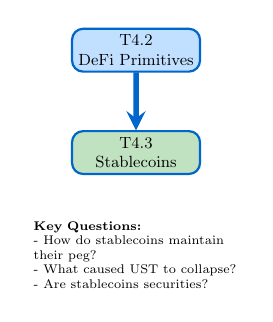
\begin{tikzpicture}[scale=0.65, transform shape]
    % Current topic
    \node[smartcontract, minimum width=2.5cm, fill=dflightblue3] (current) at (0, 2) {T4.2\\DeFi Primitives};

    % Next topic
    \node[smartcontract, minimum width=2.5cm, fill=dfgreen!30] (next) at (0, 0) {T4.3\\Stablecoins};

    % Arrow
    \draw[arrow, line width=2pt] (current) -- (next);

    % Key questions
    \node[text width=4cm, font=\scriptsize, align=left] at (0, -2) {
        \textbf{Key Questions:}\\
        - How do stablecoins maintain their peg?\\
        - What caused UST to collapse?\\
        - Are stablecoins securities?
    };
\end{tikzpicture}
\end{column}
\end{columns}

\vspace{0.2cm}
\bottomnote{Hands-on: NB10 -- Stablecoin price stability analysis}
\end{frame}

% =====================================================================
% SLIDE 40: RESOURCES
% =====================================================================
\begin{frame}{Resources for Further Learning}
\begin{columns}[T]
\begin{column}{0.48\textwidth}
\textbf{Essential Reading:}
\begin{itemize}
    \item Uniswap V2 Whitepaper
    \item Aave Documentation
    \item ``DeFi and the Future of Finance'' (Campbell Harvey)
\end{itemize}

\vspace{0.3cm}
\textbf{Interactive Tools:}
\begin{itemize}
    \item DefiLlama (TVL tracking)
    \item Dune Analytics (on-chain data)
    \item Impermanent Loss calculators
\end{itemize}
\end{column}

\begin{column}{0.48\textwidth}
\textbf{Technical Resources:}
\begin{itemize}
    \item Ethereum.org DeFi docs
    \item Curve Finance resources
    \item Chainlink education
\end{itemize}

\vspace{0.3cm}
\textbf{Stay Updated:}
\begin{itemize}
    \item The Defiant newsletter
    \item Bankless podcast
    \item Week in Ethereum News
\end{itemize}
\end{column}
\end{columns}

\vspace{0.3cm}
\begin{block}{Course Materials}
\textbf{Notebook NB09}: AMM Simulation -- practice with $x \cdot y = k$, slippage, and IL calculations
\end{block}
\end{frame}

% =====================================================================
% SLIDE 41: QUESTIONS
% =====================================================================
\begin{frame}{Questions?}
\begin{center}
\vspace{1cm}
{\Huge Topic 4.2: DeFi Primitives}

\vspace{0.5cm}
{\large Lending, AMMs, and Financial Legos}

\vspace{1cm}
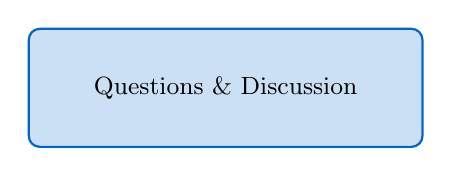
\begin{tikzpicture}
    \node[smartcontract, minimum width=5cm, minimum height=1.5cm, fill=dfblue!20] {Questions \& Discussion};
\end{tikzpicture}

\vspace{1cm}
\textbf{Next Topic:} T4.3 -- Stablecoins: The Bridge Between Two Worlds

\vspace{0.5cm}
\textcolor{dfgray}{\small Joerg Osterrieder | Digital Finance | 2025}
\end{center}
\end{frame}

\end{document}
